\section{Framework Validation}
\label{appendix:FrameworkValidation}

\begin{figure}[H]
    \centering
    \begin{subfigure}[t]{0.32\linewidth}
        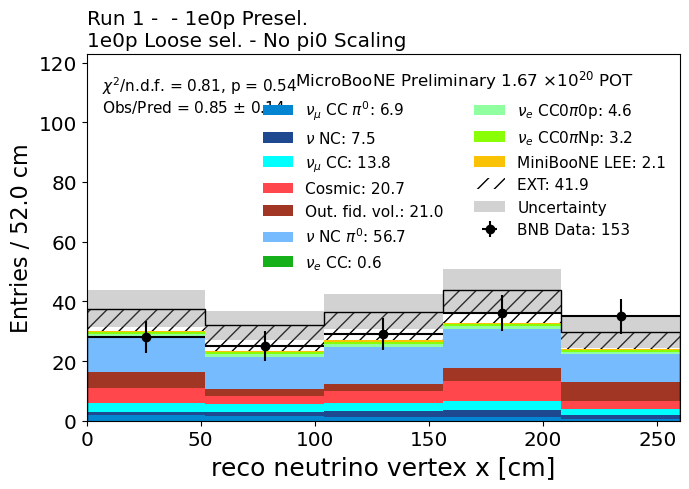
\includegraphics[width=\linewidth]{technote/Appendix_Validation/Figures/1e0p_Loose/Run1_Vertex_X_Old.png}
        \caption{Old codebase.}
    \end{subfigure}%
    \hspace{0.2cm}%
    \begin{subfigure}[t]{0.32\linewidth}
        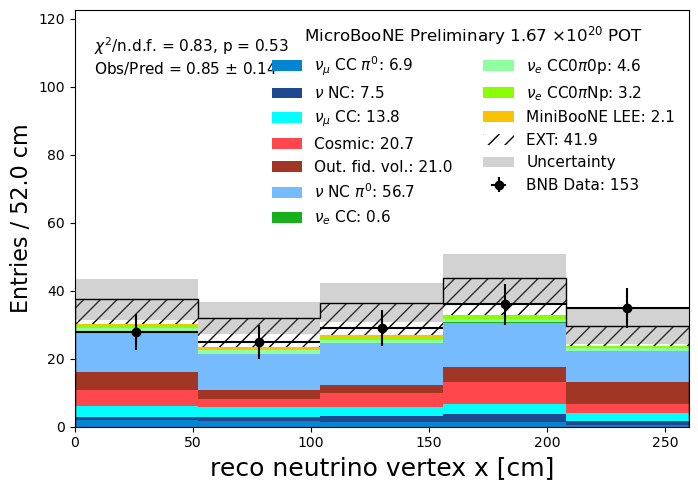
\includegraphics[width=\linewidth]{technote/Appendix_Validation/Figures/1e0p_Loose/Run1_Vertex_X_Chris.png}
        \caption{Hybrid code.}
    \end{subfigure}%
    \hspace{0.2cm}%
    \begin{subfigure}[t]{0.32\linewidth}
        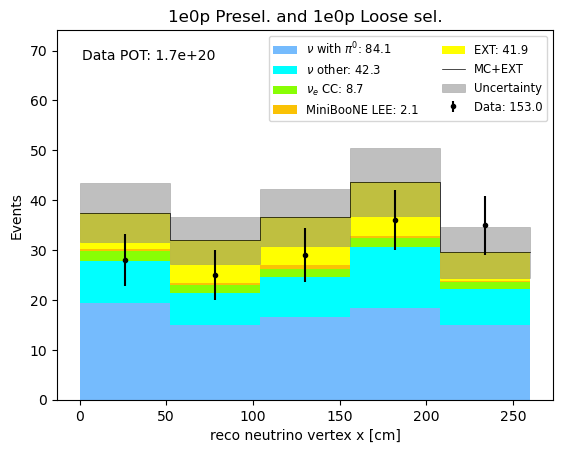
\includegraphics[width=\linewidth]{technote/Appendix_Validation/Figures/1e0p_Loose/Run1_Vertex_X_Alex.png}
        \caption{New codebase.}
    \end{subfigure}
    \caption{Validation of the new code framework using data and simulation from run 1, after application of the loose 1e0p event selection.}
\end{figure}

\begin{figure}[H]
    \centering
    \begin{subfigure}[t]{0.32\linewidth}
        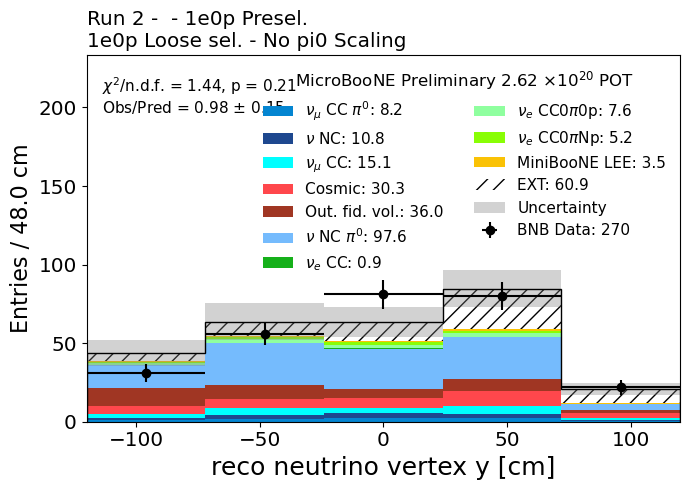
\includegraphics[width=\linewidth]{technote/Appendix_Validation/Figures/1e0p_Loose/Run2_Vertex_Y_Old.png}
        \caption{Old codebase.}
    \end{subfigure}%
    \hspace{0.2cm}%
    \begin{subfigure}[t]{0.32\linewidth}
        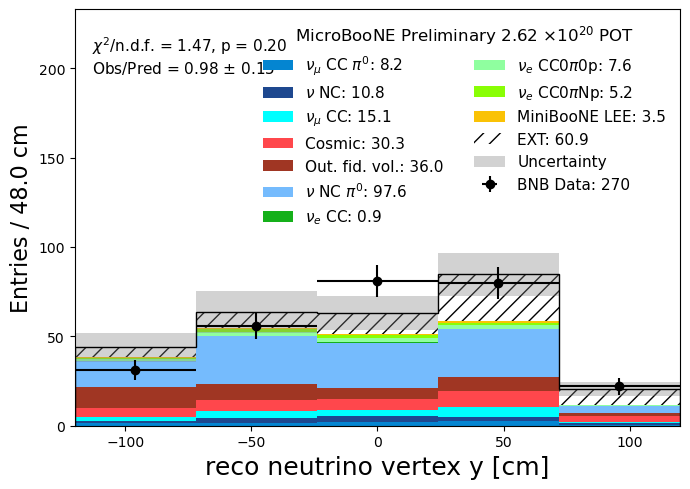
\includegraphics[width=\linewidth]{technote/Appendix_Validation/Figures/1e0p_Loose/Run2_Vertex_Y_Chris.png}
        \caption{Hybrid code.}
    \end{subfigure}%
    \hspace{0.2cm}%
    \begin{subfigure}[t]{0.32\linewidth}
        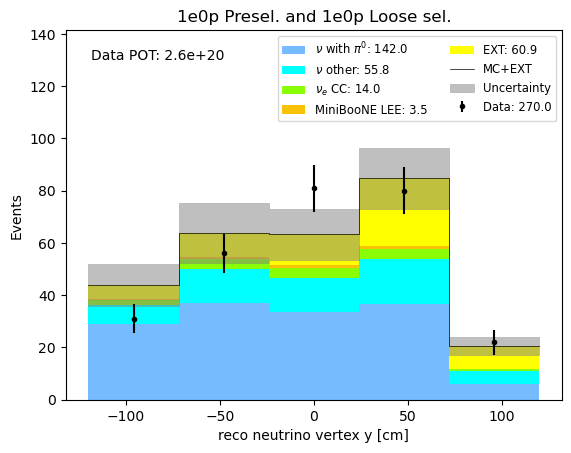
\includegraphics[width=\linewidth]{technote/Appendix_Validation/Figures/1e0p_Loose/Run2_Vertex_Y_Alex.png}
        \caption{New codebase.}
    \end{subfigure}
    \caption{Validation of the new code framework using data and simulation from run 2, after application of the loose 1e0p event selection.}
\end{figure}

\begin{figure}[H]
    \centering
    \begin{subfigure}[t]{0.32\linewidth}
        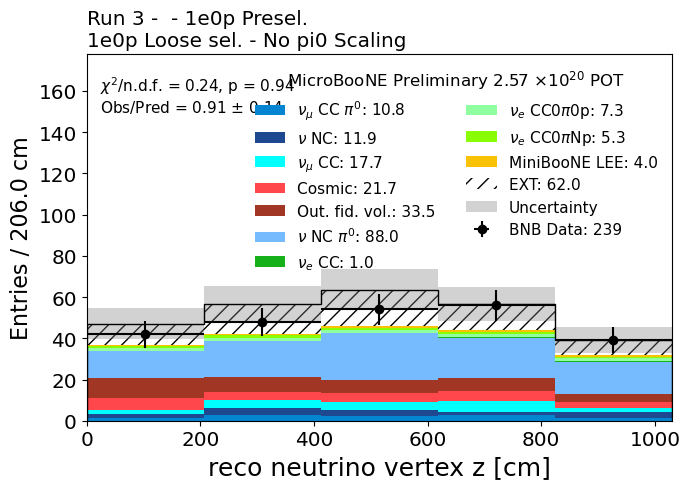
\includegraphics[width=\linewidth]{technote/Appendix_Validation/Figures/1e0p_Loose/Run3_Vertex_Z_Old.png}
        \caption{Old codebase.}
    \end{subfigure}%
    \hspace{0.2cm}%
    \begin{subfigure}[t]{0.32\linewidth}
        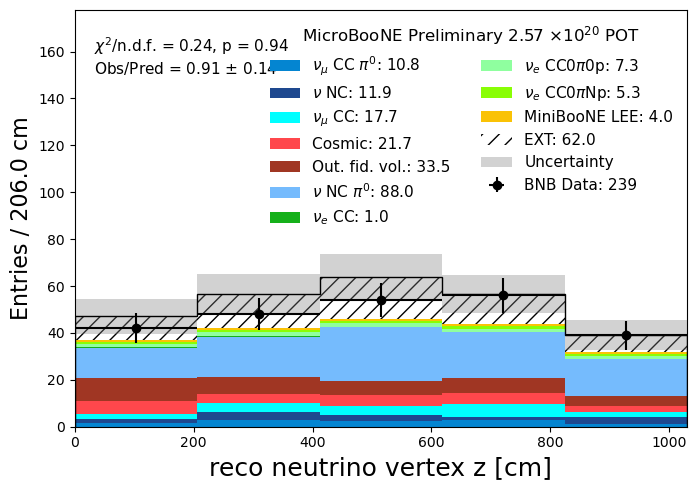
\includegraphics[width=\linewidth]{technote/Appendix_Validation/Figures/1e0p_Loose/Run3_Vertex_Z_Chris.png}
        \caption{Hybrid code.}
    \end{subfigure}%
    \hspace{0.2cm}%
    \begin{subfigure}[t]{0.32\linewidth}
        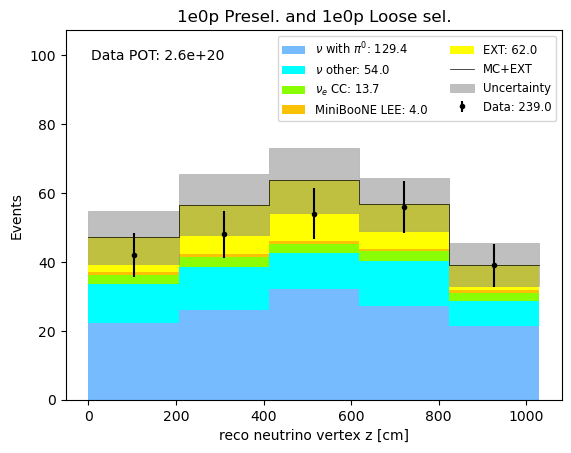
\includegraphics[width=\linewidth]{technote/Appendix_Validation/Figures/1e0p_Loose/Run3_Vertex_Z_Alex.png}
        \caption{New codebase.}
    \end{subfigure}
    \caption{Validation of the new code framework using data and simulation from run 3, after application of the loose 1e0p event selection.}
\end{figure}




\begin{figure}[H]
    \centering
    \begin{subfigure}[t]{0.32\linewidth}
        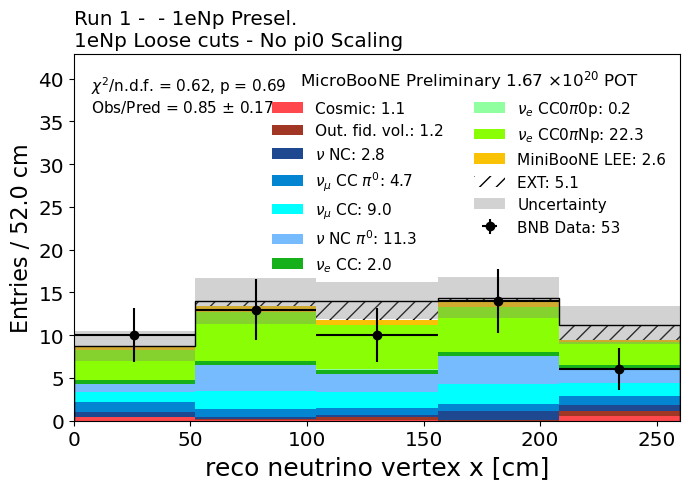
\includegraphics[width=\linewidth]{technote/Appendix_Validation/Figures/1eNp_Loose/Run1_Vertex_X_Old.png}
        \caption{Old codebase.}
    \end{subfigure}%
    \hspace{0.2cm}%
    \begin{subfigure}[t]{0.32\linewidth}
        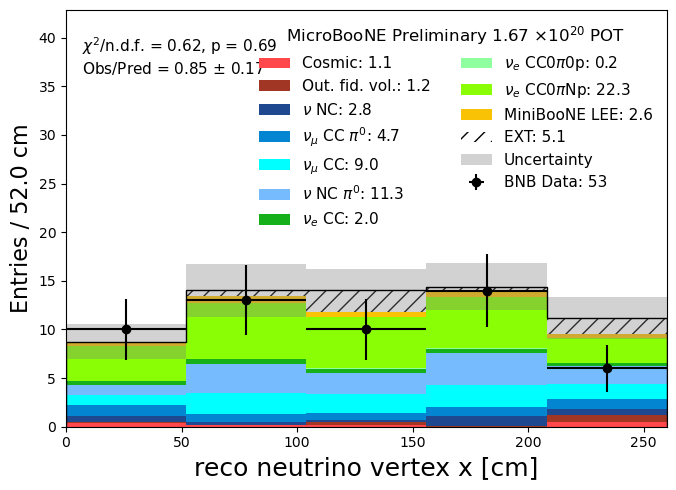
\includegraphics[width=\linewidth]{technote/Appendix_Validation/Figures/1eNp_Loose/Run1_Vertex_X_Chris.png}
        \caption{Hybrid code.}
    \end{subfigure}%
    \hspace{0.2cm}%
    \begin{subfigure}[t]{0.32\linewidth}
        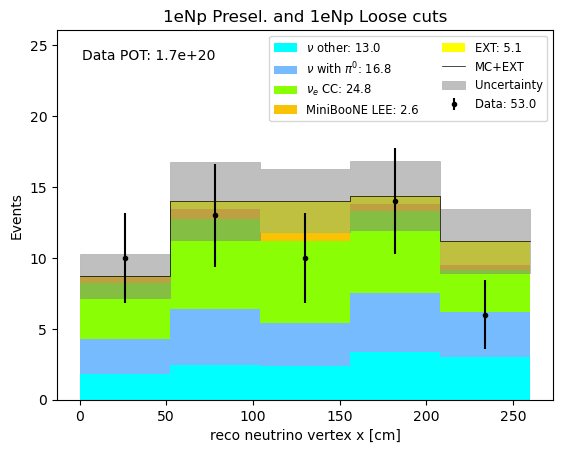
\includegraphics[width=\linewidth]{technote/Appendix_Validation/Figures/1eNp_Loose/Run1_Vertex_X_Alex.png}
        \caption{New codebase.}
    \end{subfigure}
    \caption{Validation of the new code framework using data and simulation from run 1, after application of the loose 1eNp event selection.}
\end{figure}

\begin{figure}[H]
    \centering
    \begin{subfigure}[t]{0.32\linewidth}
        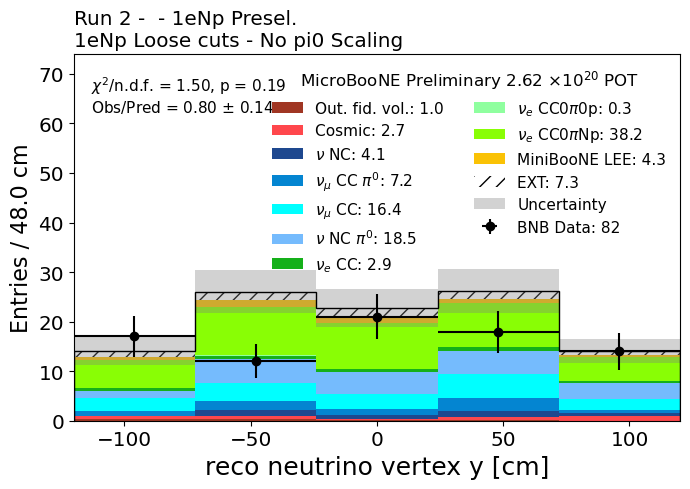
\includegraphics[width=\linewidth]{technote/Appendix_Validation/Figures/1eNp_Loose/Run2_Vertex_Y_Old.png}
        \caption{Old codebase.}
    \end{subfigure}%
    \hspace{0.2cm}%
    \begin{subfigure}[t]{0.32\linewidth}
        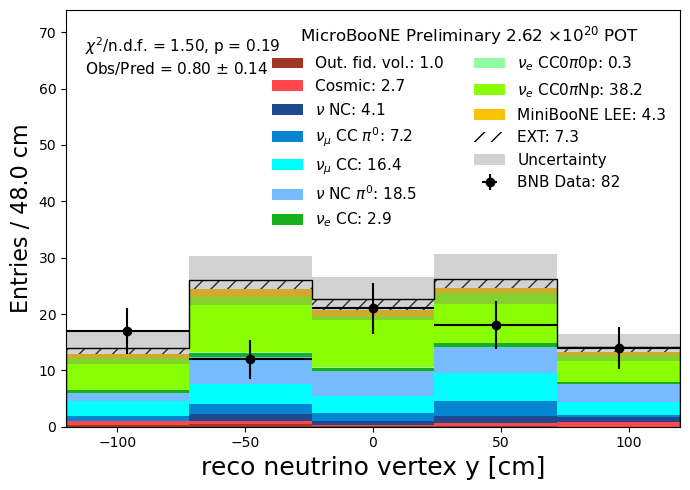
\includegraphics[width=\linewidth]{technote/Appendix_Validation/Figures/1eNp_Loose/Run2_Vertex_Y_Chris.png}
        \caption{Hybrid code.}
    \end{subfigure}%
    \hspace{0.2cm}%
    \begin{subfigure}[t]{0.32\linewidth}
        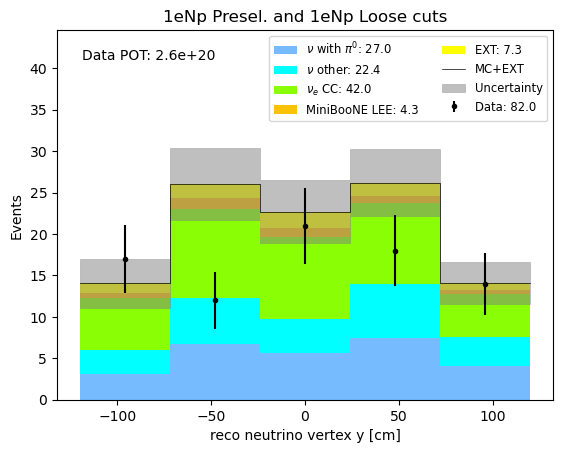
\includegraphics[width=\linewidth]{technote/Appendix_Validation/Figures/1eNp_Loose/Run2_Vertex_Y_Alex.png}
        \caption{New codebase.}
    \end{subfigure}
    \caption{Validation of the new code framework using data and simulation from run 2, after application of the loose 1eNp event selection.}
\end{figure}

\begin{figure}[H]
    \centering
    \begin{subfigure}[t]{0.32\linewidth}
        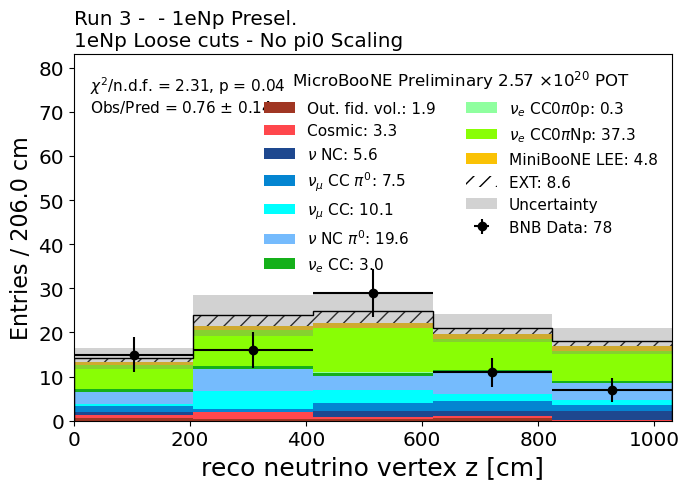
\includegraphics[width=\linewidth]{technote/Appendix_Validation/Figures/1eNp_Loose/Run3_Vertex_Z_Old.png}
        \caption{Old codebase.}
    \end{subfigure}%
    \hspace{0.2cm}%
    \begin{subfigure}[t]{0.32\linewidth}
        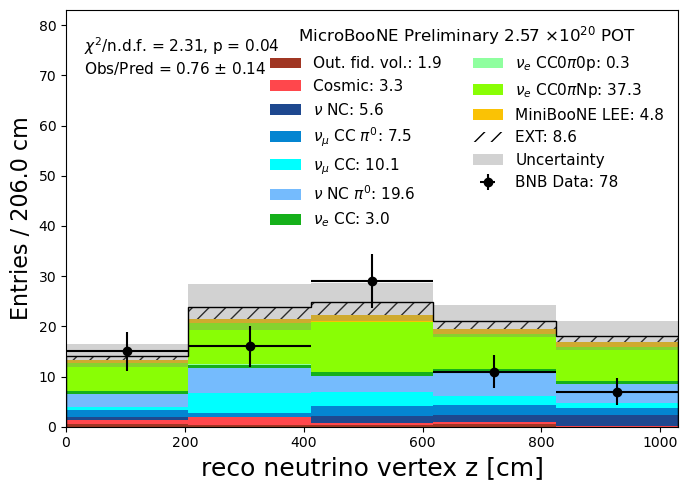
\includegraphics[width=\linewidth]{technote/Appendix_Validation/Figures/1eNp_Loose/Run3_Vertex_Z_Chris.png}
        \caption{Hybrid code.}
    \end{subfigure}%
    \hspace{0.2cm}%
    \begin{subfigure}[t]{0.32\linewidth}
        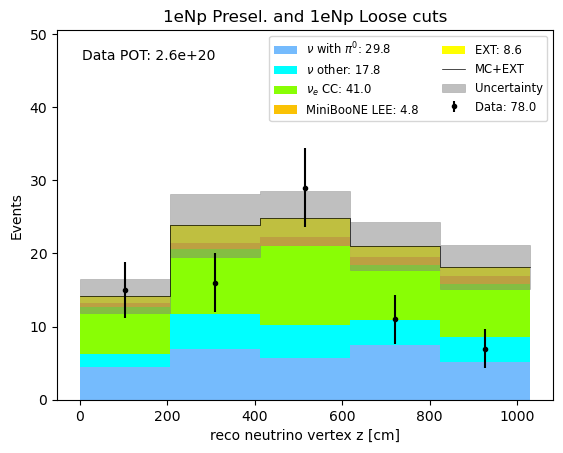
\includegraphics[width=\linewidth]{technote/Appendix_Validation/Figures/1eNp_Loose/Run3_Vertex_Z_Alex.png}
        \caption{New codebase.}
    \end{subfigure}
    \caption{Validation of the new code framework using data and simulation from run 3, after application of the loose 1eNp event selection.}
\end{figure}







\begin{figure}[H]
    \centering
    \begin{subfigure}[t]{0.32\linewidth}
        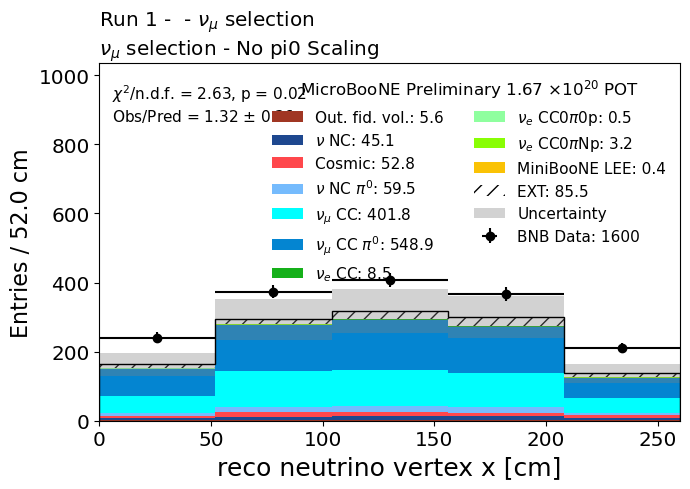
\includegraphics[width=\linewidth]{technote/Appendix_Validation/Figures/Numu/Run1_Vertex_X_Old.png}
        \caption{Old codebase.}
    \end{subfigure}%
    \hspace{0.2cm}%
    \begin{subfigure}[t]{0.32\linewidth}
        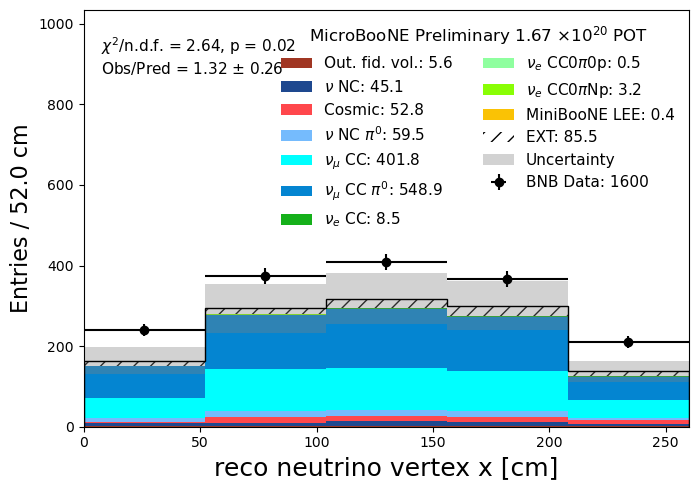
\includegraphics[width=\linewidth]{technote/Appendix_Validation/Figures/Numu/Run1_Vertex_X_Chris.png}
        \caption{Hybrid code.}
    \end{subfigure}%
    \hspace{0.2cm}%
    \begin{subfigure}[t]{0.32\linewidth}
        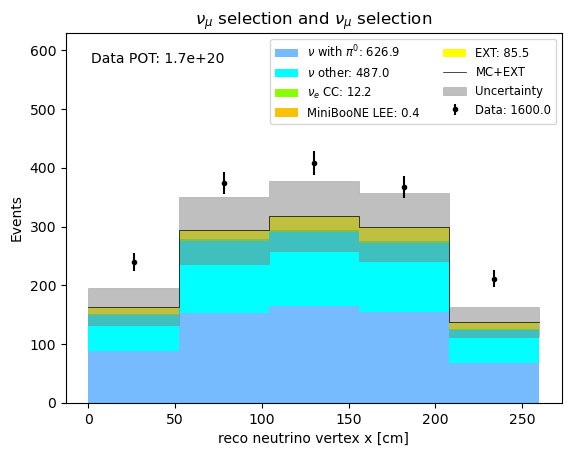
\includegraphics[width=\linewidth]{technote/Appendix_Validation/Figures/Numu/Run1_Vertex_X_Alex.png}
        \caption{New codebase.}
    \end{subfigure}
    \caption{Validation of the new code framework using data and simulation from run 1, after application of the loose $\nu_{\mu}$ event selection.}
\end{figure}

\begin{figure}[H]
    \centering
    \begin{subfigure}[t]{0.32\linewidth}
        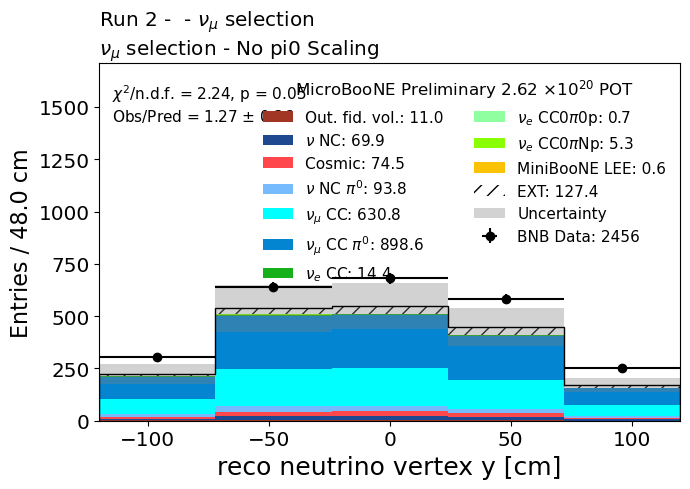
\includegraphics[width=\linewidth]{technote/Appendix_Validation/Figures/Numu/Run2_Vertex_Y_Old.png}
        \caption{Old codebase.}
    \end{subfigure}%
    \hspace{0.2cm}%
    \begin{subfigure}[t]{0.32\linewidth}
        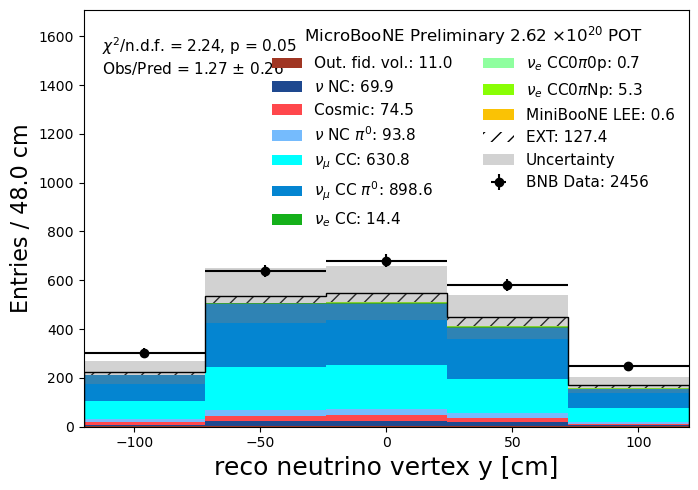
\includegraphics[width=\linewidth]{technote/Appendix_Validation/Figures/Numu/Run2_Vertex_Y_Chris.png}
        \caption{Hybrid code.}
    \end{subfigure}%
    \hspace{0.2cm}%
    \begin{subfigure}[t]{0.32\linewidth}
        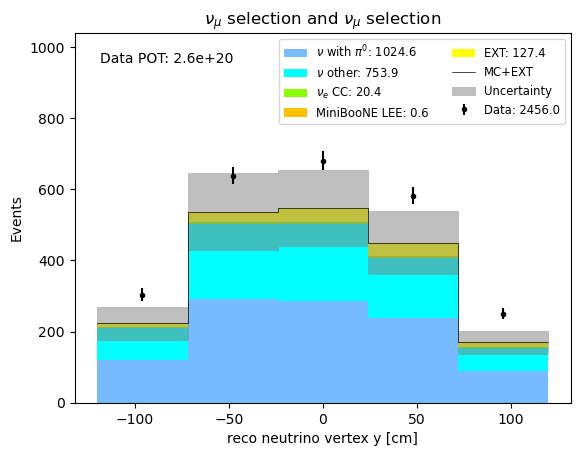
\includegraphics[width=\linewidth]{technote/Appendix_Validation/Figures/Numu/Run2_Vertex_Y_Alex.png}
        \caption{New codebase.}
    \end{subfigure}
    \caption{Validation of the new code framework using data and simulation from run 2, after application of the $\nu_{\mu}$ event selection.}
\end{figure}

\begin{figure}[H]
    \centering
    \begin{subfigure}[t]{0.32\linewidth}
        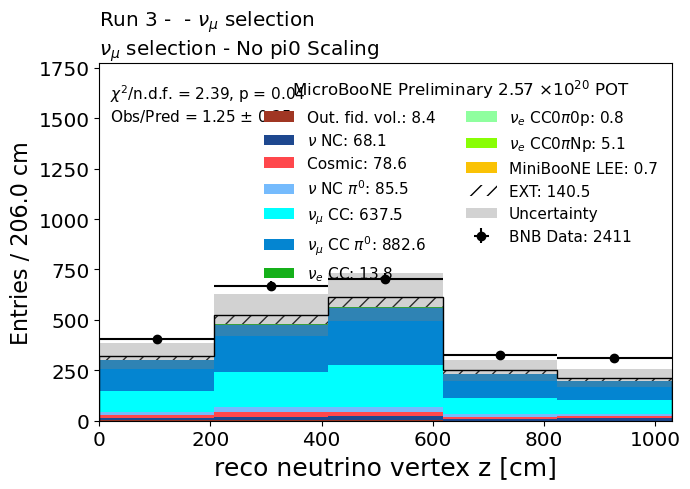
\includegraphics[width=\linewidth]{technote/Appendix_Validation/Figures/Numu/Run3_Vertex_Z_Old.png}
        \caption{Old codebase.}
    \end{subfigure}%
    \hspace{0.2cm}%
    \begin{subfigure}[t]{0.32\linewidth}
        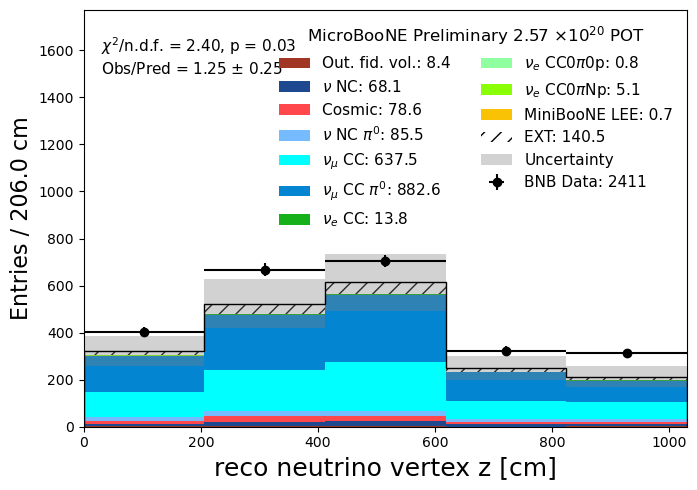
\includegraphics[width=\linewidth]{technote/Appendix_Validation/Figures/Numu/Run3_Vertex_Z_Chris.png}
        \caption{Hybrid code.}
    \end{subfigure}%
    \hspace{0.2cm}%
    \begin{subfigure}[t]{0.32\linewidth}
        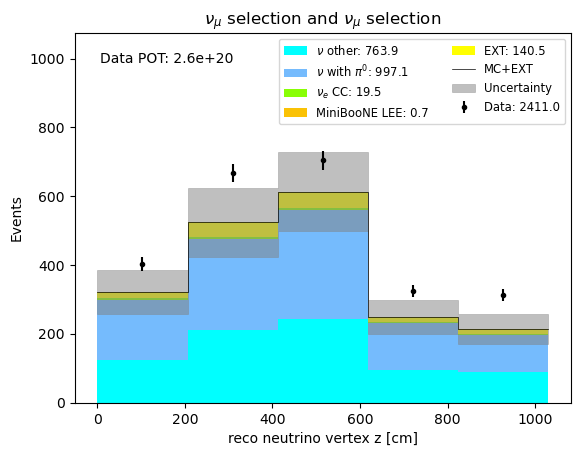
\includegraphics[width=\linewidth]{technote/Appendix_Validation/Figures/Numu/Run3_Vertex_Z_Alex.png}
        \caption{New codebase.}
    \end{subfigure}
    \caption{Validation of the new code framework using data and simulation from run 3, after application of the $\nu_{\mu}$ event selection.}
\end{figure}
